\section{Module 3: Máy ảo Đa Card mạng \& Xử lý Định tuyến Bất đối xứng}

\subsection{Mục tiêu \& Thách thức Kiến trúc Định tuyến}
Trong Module 3, nhóm chúng em triển khai một máy ảo đóng vai trò Application Gateway gắn đồng thời vào cả hai phân đoạn mạng DMZ và Private. Trong quá trình thực nghiệm các hệ thống đa card mạng (Multi-Homed), một thách thức kỹ thuật lớn mà nhóm gặp phải chính là hiện tượng \textbf{định tuyến bất đối xứng} (Asymmetric Routing, mô tả tại Hình~\ref{fig:m3_asymm_concept}): gói tin yêu cầu chiều vào (Ingress) được gửi tới Floating IP và đi qua cổng DMZ, nhưng gói tin phản hồi chiều ra (Egress) lại bị hệ điều hành gửi nhầm qua cổng Private theo bảng định tuyến mặc định. Kết quả là tường lửa kiểm tra trạng thái (Stateful Firewall/Conntrack) trên Neutron Router coi đây là luồng gói tin không hợp lệ và lập tức hủy bỏ (drop) kết nối.

\begin{figure}[H]
\centering
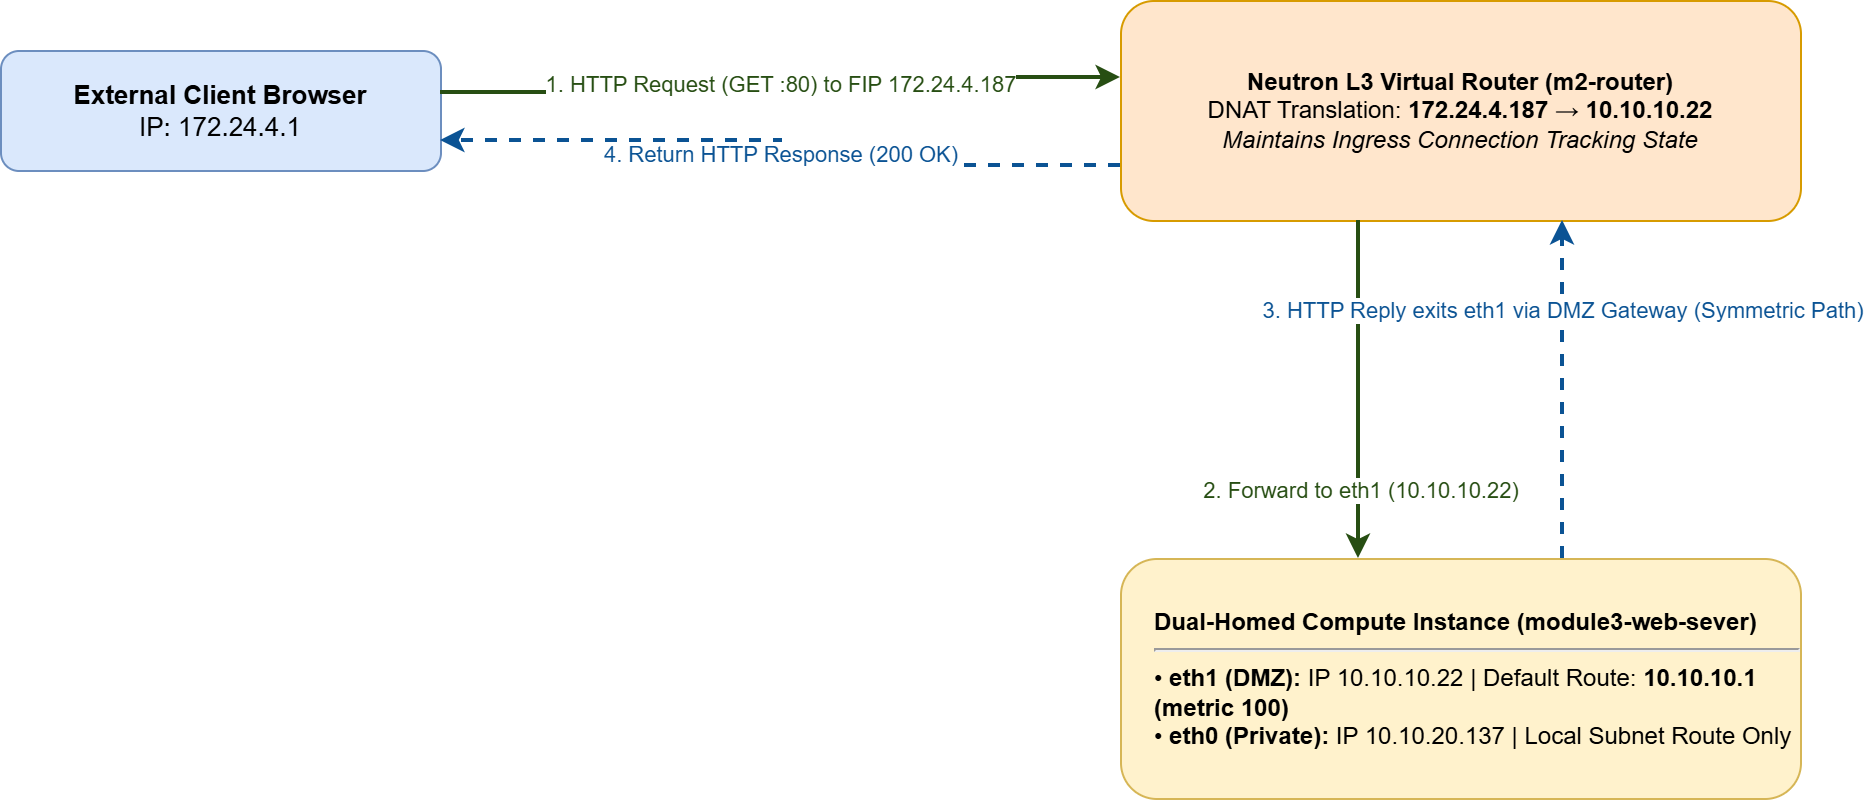
\includegraphics[width=0.92\linewidth]{img/routing_traffic_flow.png}
\caption{Luồng gói tin Ingress và Egress của máy ảo web đa card mạng dưới sự kiểm soát định tuyến đối xứng.}
\label{fig:m3_asymm_concept}
\end{figure}

\subsection{Quy trình Triển khai}
Nhóm chúng em thực hiện quy trình triển khai theo các bước sau:
\begin{enumerate}
    \item \textbf{Khởi tạo Nhóm Bảo mật (\texttt{module3-web-sg}):}
    Nhóm thiết lập Security Group chuyên biệt với các luật cho phép lưu lượng SSH (TCP cổng 22), HTTP (TCP cổng 80) và giao thức ICMP (Ping) từ mọi dải địa chỉ IPv4 (\nolinkurl{0.0.0.0/0}), như minh họa tại Hình~\ref{fig:m3_secgroup_rules}.
    
    \item \textbf{Khởi tạo Máy ảo 2 Card mạng (\texttt{module3-web-sever}) (Hình~\ref{fig:m3_instance_overview}):}
    Trước khi khởi tạo máy ảo, nhóm tiến hành xác thực lại danh mục mạng tenant để đảm bảo gán đúng giao diện (Hình~\ref{fig:m3_networks_verify}). Sau đó, máy ảo được khởi chạy với 2 cổng mạng ảo chuyên dụng:
    \begin{itemize}
        \item \textbf{NIC 1 (\texttt{eth1}):} Gắn vào phân vùng \texttt{m2-dmz-net} với địa chỉ IP tĩnh \texttt{10.10.10.22}.
        \item \textbf{NIC 2 (\texttt{eth0}):} Gắn vào phân vùng \texttt{m2-private-net} với địa chỉ IP tĩnh \texttt{10.10.20.137}.
    \end{itemize}

    \item \textbf{Gán Địa chỉ IP Nổi (Floating IP):}
    Nhóm xin cấp phát địa chỉ IP công khai \texttt{172.24.4.187} từ pool mạng \texttt{public} và thực hiện ánh xạ \textbf{chính xác vào cổng DMZ} (\texttt{10.10.10.22}) thay vì cổng Private (Hình~\ref{fig:m3_floating_ip}).
\end{enumerate}

\begin{figure}[H]
\centering
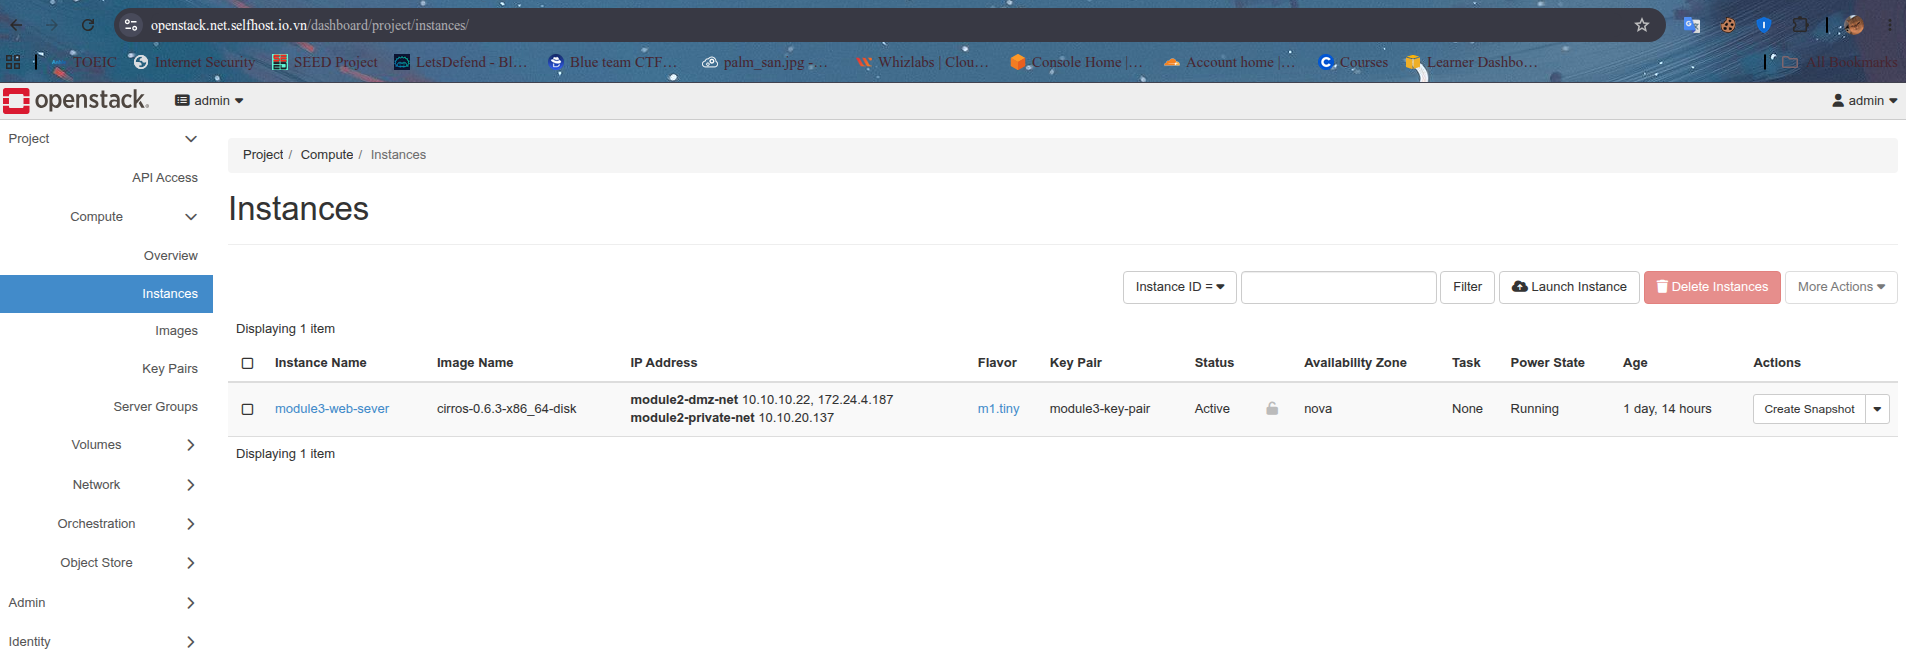
\includegraphics[width=0.88\linewidth]{img/m3-instance-dual-homed-overview.png}
\caption{Máy ảo \texttt{module3-web-sever} gắn đồng thời 2 card mạng DMZ và Private.}
\label{fig:m3_instance_overview}
\end{figure}

\begin{figure}[H]
\centering
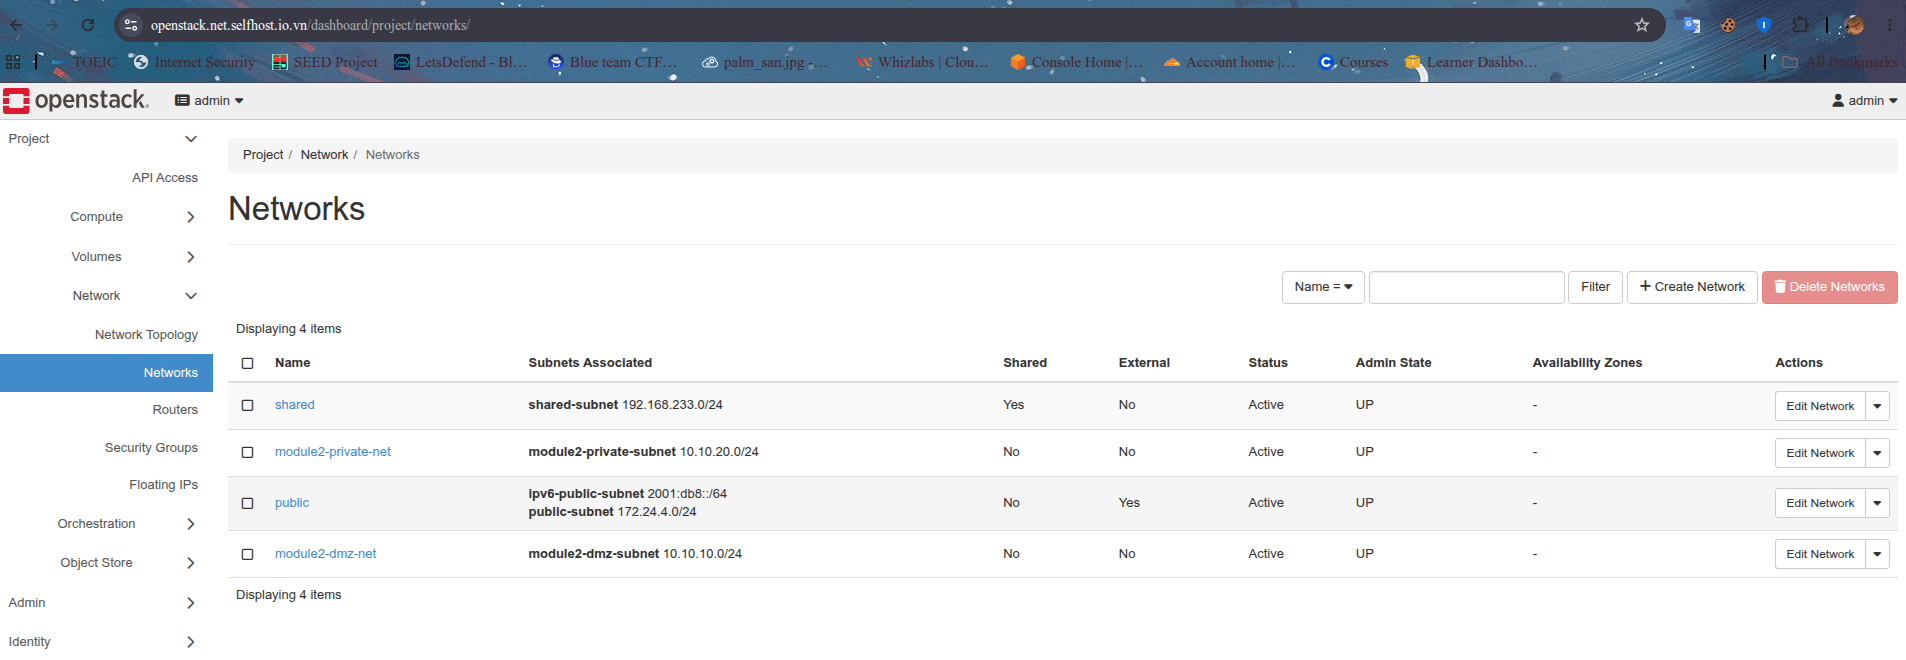
\includegraphics[width=0.88\linewidth]{img/m3-network-inventory.png}
\caption{Xác nhận bảng danh mục mạng tenant trước khi đính kèm máy ảo.}
\label{fig:m3_networks_verify}
\end{figure}

\begin{figure}[H]
\centering
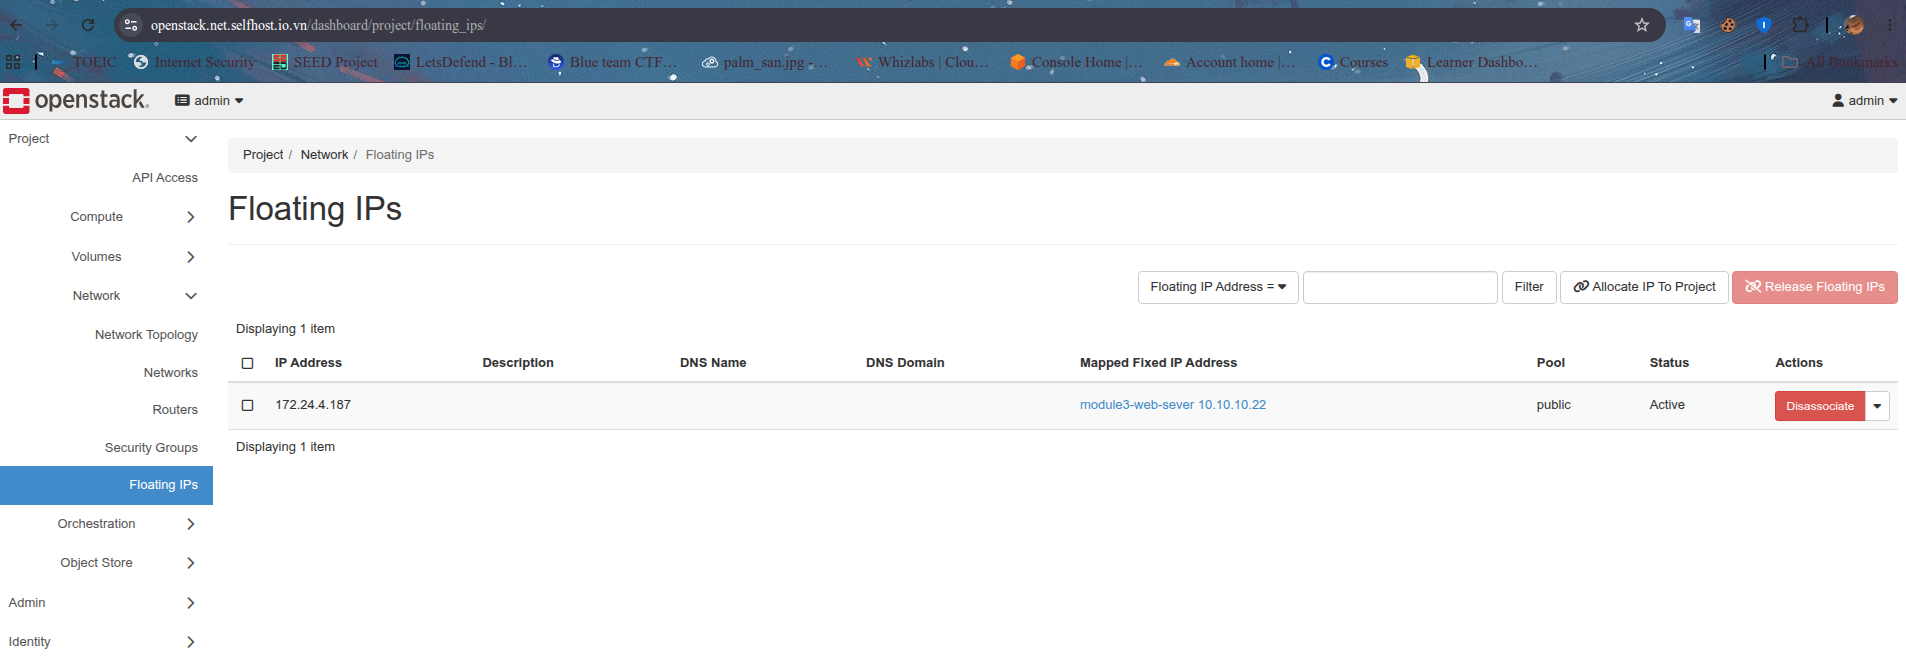
\includegraphics[width=0.88\linewidth]{img/m3-floating-ip-mapping.png}
\caption{Floating IP \texttt{172.24.4.187} ánh xạ chính xác vào IP cố định DMZ \texttt{10.10.10.22}.}
\label{fig:m3_floating_ip}
\end{figure}

\begin{figure}[H]
\centering
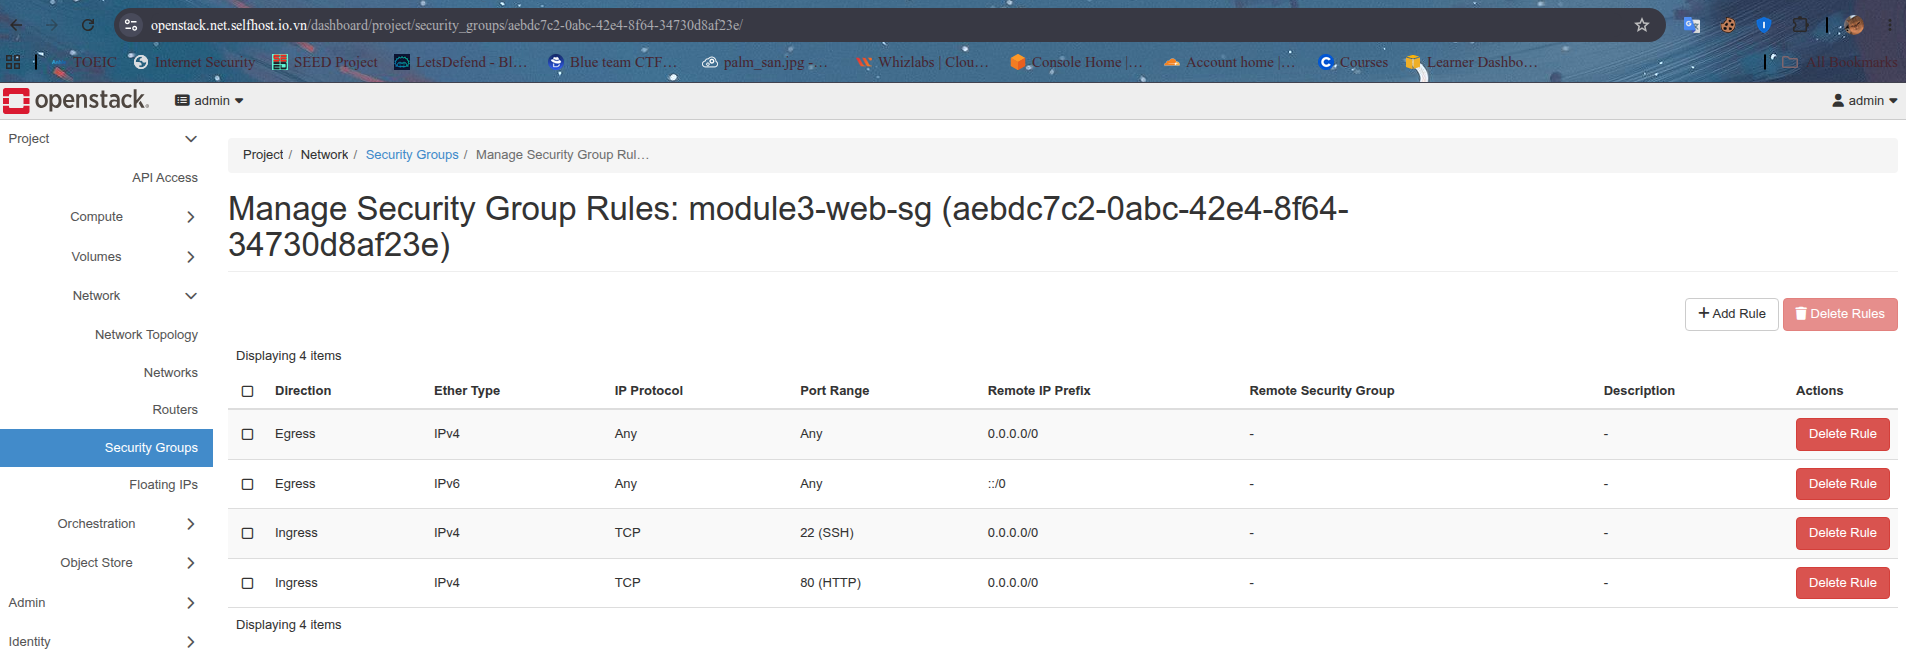
\includegraphics[width=0.88\linewidth]{img/m3-security-group-rules.png}
\caption{Luật tường lửa Security Group \texttt{module3-web-sg} mở các cổng 22, 80 và ICMP.}
\label{fig:m3_secgroup_rules}
\end{figure}

\subsection{Cấu hình Bảng Định tuyến Kernel \& Kiểm thử Dịch vụ Web}
Sau khi truy cập vào console của máy ảo qua SSH, nhóm chúng em kiểm tra thông số mạng và phát hiện vấn đề định tuyến thực tế (Hình~\ref{fig:m3_ip_route}):
\begin{itemize}
    \item Qua lệnh \texttt{ip addr}, nhóm xác nhận cổng \texttt{eth0} nhận địa chỉ \nolinkurl{10.10.20.137/24} (Private) và cổng \texttt{eth1} nhận địa chỉ \nolinkurl{10.10.10.22/24} (DMZ).
    \item Tuy nhiên, DHCP mặc định đã thiết lập Default Gateway trỏ qua giao diện \texttt{eth0} (mạng Private). Để xử lý triệt để hiện tượng định tuyến bất đối xứng và tránh bị Router hủy gói tin do lệch phiên theo dõi conntrack, nhóm chúng em đã cấu hình lại bảng định tuyến của nhân Linux nhằm ưu tiên Default Gateway đi qua cổng DMZ:
\begin{lstlisting}[language=bash]
$ sudo ip route replace default via 10.10.10.1 dev eth1 metric 100
\end{lstlisting}
    Quy tắc này bảo đảm mọi gói tin phản hồi ra bên ngoài (đặc biệt là lưu lượng HTTP) đều bắt buộc đi ngược lại qua cổng DMZ (\texttt{eth1}), nơi bảng phiên dịch địa chỉ (DNAT/SNAT) của Neutron Router đang duy trì trạng thái phiên.
\end{itemize}

\begin{figure}[H]
\centering
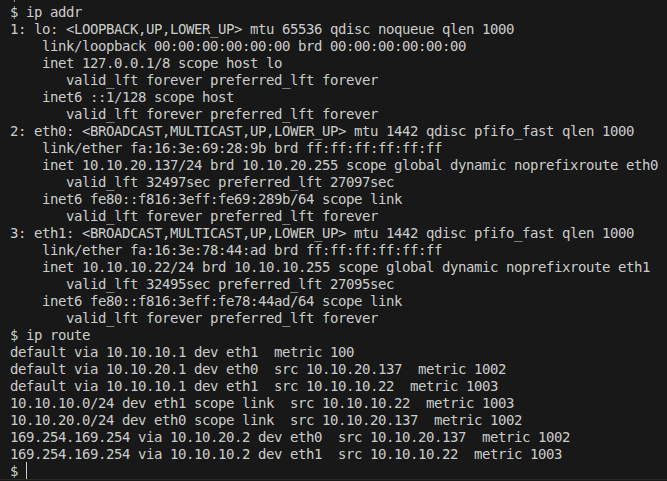
\includegraphics[width=0.88\linewidth]{img/m3-instance-ip-route-terminal.png}
\caption{Cấu hình mạng nội bộ máy ảo (\texttt{ip addr}) và bảng định tuyến kernel (\texttt{ip route}).}
\label{fig:m3_ip_route}
\end{figure}

\noindent \textbf{Khởi chạy Dịch vụ \& Nghiệm thu Toàn trình:}
Để kiểm thử khả năng cung cấp dịch vụ web ra ngoài Internet, nhóm chúng em khởi chạy web server bằng lệnh \texttt{sudo busybox httpd -f -p 80 -v}. Từ máy client bên ngoài, nhóm tiến hành gửi yêu cầu HTTP đến địa chỉ Floating IP \url{http://172.24.4.187}. Kết quả thực nghiệm ghi nhận nhật ký truy cập (access log) hiển thị đầy đủ trên terminal của máy chủ (Hình~\ref{fig:m3_busybox_logs}), đồng thời giao diện web được tải và render thành công trên trình duyệt của máy khách (Hình~\ref{fig:m3_browser_http}), chứng minh giải pháp xử lý định tuyến đối xứng hoạt động hoàn toàn chính xác.

\begin{figure}[H]
\centering
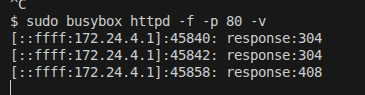
\includegraphics[width=0.88\linewidth]{img/m3-busybox-httpd-logs.png}
\caption{Nhật ký truy cập của tiến trình BusyBox HTTP daemon ghi nhận yêu cầu từ client.}
\label{fig:m3_busybox_logs}
\end{figure}

\begin{figure}[H]
\centering
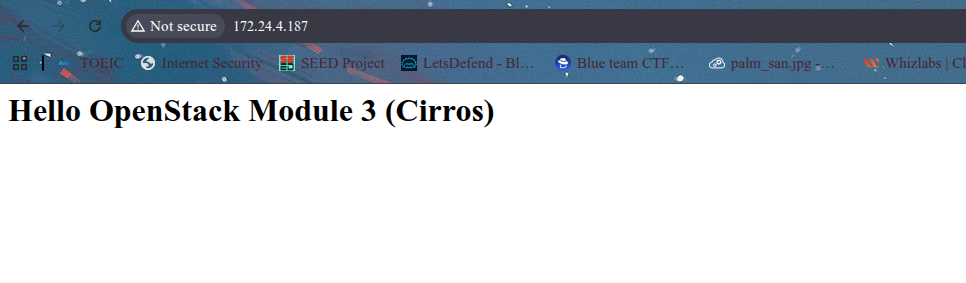
\includegraphics[width=0.88\linewidth]{img/m3-web-browser-http-verification.png}
\caption{Kiểm thử truy cập dịch vụ web thành công qua trình duyệt với Floating IP \texttt{172.24.4.187}.}
\label{fig:m3_browser_http}
\end{figure}
